\chapter{GE11 detector generations} % (fold)
\label{cha:ge11_detector_generations}
\begin{figure}[!htbp]
	\centering
	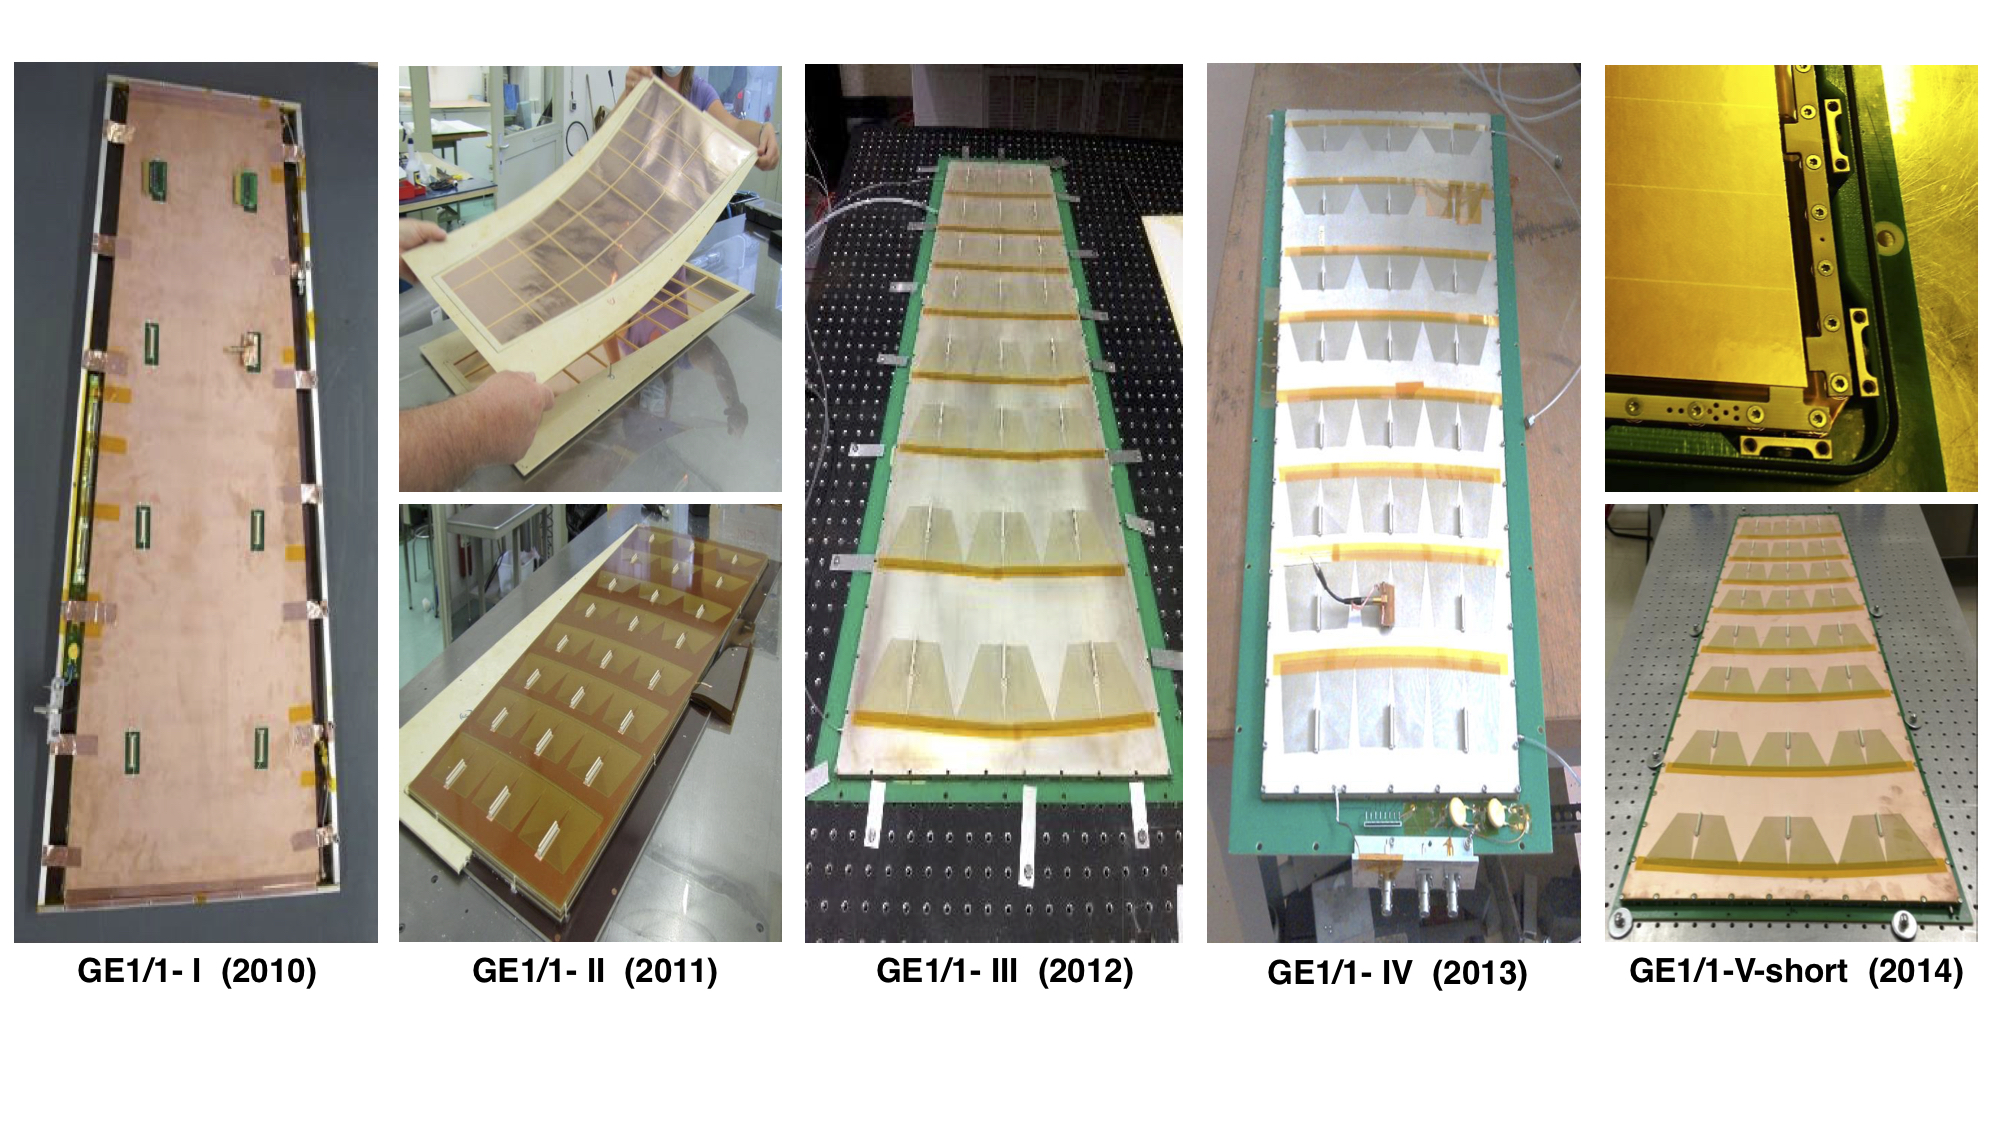
\includegraphics[width=0.95\textwidth]{figures/GEM/5-prototype-generations.jpg}
	\caption{Five different generations of GE11 detector developed and improved with time.}
	\label{fig:GE11generations}
\end{figure}
From 2010 till now total of five different GE11 versions are developed and tested every year. Based on the experience every new generation was improved from its previous versions.

In the first version of GE11, GE11-I, prototype was build 1m-class GEM detector and operated. In this detector different components are glued together and to have gaps between different GEMs spacer ribs were used to have the gap configurations 3/2/2/2 mm. In this version total 8 readout sector was there~\cite{Abbaneo2010}.

In the next version, GE11-II, the readout sectors were increased from 8 to 24 which are arranged as 8-$\eta$ partitions and 3-$\phi$ partition (columns). Here, each $\eta$ partitions had 384 radial strips with 455 $\mu rad$ angular pitch. Also, to speed up the signal, the foil gap configurations are changed to 3/1/2/1 mm~\cite{Abbaneo2011}.

In the third version of GE11, known as GE11-III. In this version it was split into several pieces and used the mechanical stretching during the assembly then glued to the frame and drift board~\cite{Abbaneoo2012}.

In the fourth version of GE11, GE11-IV, the major achievement was to abandoned the use of glue while assembling the detector. Because of this the stretching improved and the board deformation issue was resolved as compared to the GE11-III. Still it takes few hour in assembling and need to use the pre-bending of the with respect to the bowing observed. Thus, it was not reliable for the mass production~\cite{Abbaneo2013}. 

The pre-bending issue is resolved in the GE11-V prototype by tensioning the foil against the independent ``\textit{pull-out}'' pieces. This version is opted for the final production of the GE11 chamber for installation in the CMS during Long-Shut-down-2.

% chapter ge11_detector_generations (end)